\begin{figure}[b!]
    \centering
    \begin{tabularx}{\linewidth}{>{\centering\arraybackslash}X}
        % Fila 1: imagen
        \begin{subfigure}[t]{0.5\linewidth}
            \centering
            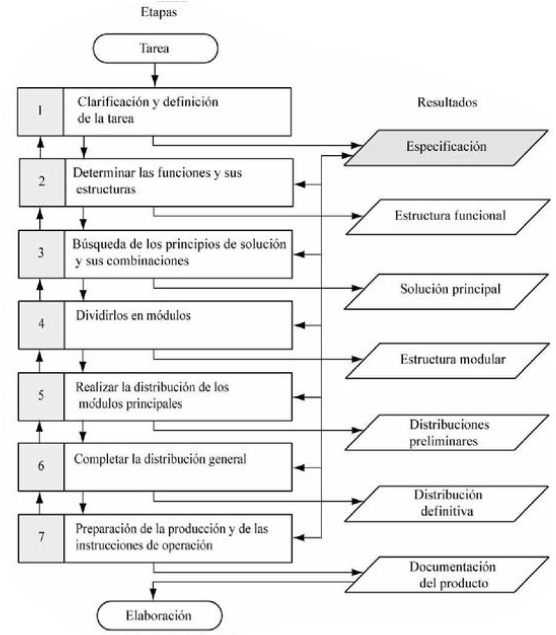
\includegraphics[width=\linewidth]{ANNEX/Fig/AB/AB_VDI2221.PNG}
        \end{subfigure}
        \\[2mm]
        % Fila 2: nota
        \begin{subfigure}[t]{\linewidth}
            \caption*{\textit{Nota: Figura adaptada de \autocite{vdi2221}.}}
        \end{subfigure}
    \end{tabularx}
    \caption{Proceso Generalizado de Desarrollo y Diseño VDI 2221}
    \label{fig:vdi2221}
\end{figure}
La primera metodología mencionada se estructura en siete fases principales que permiten abordar el proceso de diseño de manera organizada y estructurada. La primera fase se enfoca en los requerimientos de diseño, etapa que es revisada y modificada recurrentemente a lo largo del desarrollo, como se observa en el diagrama de flujo de la Figura \ref{fig:vdi2221}. La segunda etapa implica la creación de un diagrama de funciones del sistema, permitiendo una clara comprensión del funcionamiento esperado del producto. En la tercera etapa, se realiza una matriz morfológica que presenta tres posibles soluciones para cada función del sistema; estas soluciones se evalúan tanto técnica como económicamente, y la que obtiene el mejor puntaje es seleccionada. En la cuarta etapa, el producto se divide en módulos realizables, clasificándose según las áreas de mecánica, electrónica y software, debido a la naturaleza mecatrónica del diseño. La quinta etapa comprende la creación de diagramas o bosquejos preliminares de los módulos, los cuales se finalizarán en la sexta fase. Finalmente, la séptima etapa se centra en la documentación, construcción y pruebas del producto \autocite{vdi2221}.

Por otro lado, la segunda en mención,  VDI 2206, se aplica específicamente a sistemas mecatrónicos y complementa la VDI 2221. Se organiza en una estructura en forma de V como se muestra en la Figura \ref{fig:vdi2206}, donde el diseño avanza desde los requerimientos del sistema hasta la comprobación y validación del producto. En este modelo, se descomponen las funciones del sistema, las cuales se desarrollan en paralelo para los dominios mecánico, eléctrico e informáticos. A medida que el sistema avanza hacia la integración, se validan los conceptos de solución mediante pruebas y análisis, asegurando que el diseño cumpla con los requisitos establecidos en un inicio, lo cual resulta en un diseño iterativo hasta conseguir cumplir con todos los requerimientos acordados.
\begin{figure}[H]
    \centering
    \begin{tabularx}{\linewidth}{>{\centering\arraybackslash}X}
        % Fila 1: imagen
        \begin{subfigure}[t]{0.5\linewidth}
            \centering
            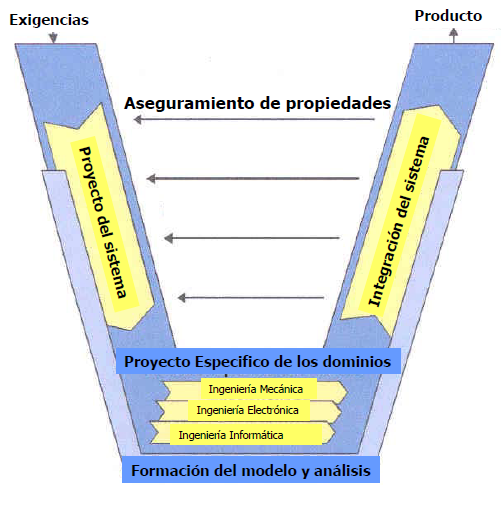
\includegraphics[width=\linewidth]{ANNEX/Fig/AB/AB_VDI2206.PNG}
        \end{subfigure}
    \end{tabularx}
    \caption{Modelo V propuesto en la norma VDI 2206}
    \label{fig:vdi2206}
\end{figure}
